% chapters/partial_solutions.tex
% 部分问题解答 (Partial Solutions of the Problems)
% 源: 原书 PDF 第 525--586 页 (印刷页 521--582)

\chapter*{部分问题解答}
\addcontentsline{toc}{chapter}{部分问题解答}
\markboth{部分问题解答}{部分问题解答}

\problemsolutionhead{1}

5. 鉴于 Zorn 引理 (引理  \ref{lem:1.1}), 只须验证 $\mathcal{F}$ 是归纳的.设 $(A_i)_{i\in I}$
为 $\mathcal{F}$ 的全序子集.令 $A=\bigcap_{i\in I}A_i$, 验证 $A$ 非空, $A$ 是 $K$ 的
极端集, $A\in\mathcal{F}$, 且 $A$ 是 $(A_i)_{i\in I}$ 的上界.

6. 反设存在 $M_0$ 中的两个相异点 $a,b$.由 Hahn--Banach 定理 (定理  \ref{thm:1.7}), 存在
某个 $f\in E^\star$ 使得 $\dual{f}{a}\ne\dual{f}{b}$.令
\begin{equation*}
M_1=\left\{x\in M_0;\ \dual{f}{x}=\max_{y\in M_0}\dual{f}{y}\right\}.
\end{equation*}
显然 $M_1\in\mathcal{F}$ 且 $M_0\le M_1$.由于 $M_0$ 极大, 推出 $M_1=M_0$.这是荒谬的,
因为点 $a$ 与 $b$ 不能同时属于 $M_1$.

8. 设 $K_1$ 为 $K$ 的所有极值点的闭凸包.反设存在某个点 $a\in K$ 使得 $a\notin K_1$.
则存在严格分离 $\{a\}$ 与 $K_1$ 的超平面.设 $f\in E^\star$ 使得对一切 $x\in K_1$,
$\dual{f}{x}<\dual{f}{a}$.注意
\begin{equation*}
B=\left\{x\in K;\ \dual{f}{x}=\max_{y\in K}\dual{f}{y}\right\}
\end{equation*}
是 $K$ 的满足 $B\cap K_1=\emptyset$ 的极端集.但 $B$ 包含 $K$ 的至少一个极值点; 矛盾.

9. (a) $\mathcal{E}=\{x=(x_i);\ \abs{x_i}=1\ \forall i\}$,

(b) $\mathcal{E}=\{x=(x_i);\ \abs{x_i}=1\ \forall i,\ \text{且对大的}\ i,\ x_i\ \text{平稳}\}$,

(c) $\mathcal{E}=\emptyset$,

(d) $\mathcal{E}=\{x=(x_i);\ \exists j\ \text{使}\ \abs{x_j}=1,\ \text{且对一切}\ i\ne j,\ x_i=0\}$,

(e) $\mathcal{E}=\{x=(x_i);\ \sum\abs{x_i}^p=1\}$,

(f) $\mathcal{E}=\emptyset$.为看出情形 (f) 中 $\mathcal{E}=\emptyset$, 设 $f\in L^1(\R)$
为满足 $\int_\R\abs{f}=1$ 的任意函数.经平移后总可以假设 $\int_{-\infty}^0\abs{f}=\int_0^\infty\abs{f}=1/2$.
然后写出 $f=(g+h)/2$, 其中在 $(-\infty,0)$ 上 $g=2f$, 在 $(0,+\infty)$ 上 $g=0$;
在 $(-\infty,0)$ 上 $h=0$, 在 $(0,+\infty)$ 上 $h=2f$.

\problemsolutionhead{2}

确定对由 $x\ge0$ 时 $\varphi(x)=-\sqrt{x}$, $x<0$ 时 $\varphi(x)=+\infty$ 定义的函数
$\varphi$ 的 $\partial\varphi(x)$.

\runin{-- A --}

4. (a) $\partial\varphi(x)=F(x)$,

(b) 当 $x\ne0$ 时 $\partial\varphi(x)=\dfrac{1}{\norm{x}}F(x)$, 且 $\partial\varphi(0)=B_{E^\star}$,

(c) 若 $x\in\operatorname{Int}K$, $\partial\varphi(x)=\{0\}$; 若 $x\in\partial K$,
$\partial\varphi(x)$ 为 $K$ 在 $x$ 处的外法锥; 若 $K$ 是线性子空间, $\partial\varphi(x)=K^\perp$,

(d) $\partial\varphi(x)=D\varphi(x)=\varphi\ \text{在}\ x\ \text{处的微分}$.

5. 研究下述例子: 在 $E=\R^2$ (配以 Euclidean 范数) 中, $\varphi=I_C$, 其中
$C=\{[x_1,x_2];\ (x_1-1)^2+x_2^2\le1\}$, 以及 $\psi=I_D$, 其中 $D=\{[x_1,x_2];\ x_1=0\}$.

\runin{-- B --}

1. 设 $C=\operatorname{epi}\varphi$.对 $A=\operatorname{Int}C$ 与 $B=[x_0,\varphi(x_0)]$
应用 Hahn--Banach 定理 (第一几何形式).注意 $A\ne\emptyset$ (为什么?).因此存在某个
$f\in E^\star$ 与常数 $k$ 与 $a$, 满足 $\norm{f}+\abs{k}\ne0$, 使得对一切 $x\in D(\varphi)$
及一切 $\lambda\ge\varphi(x)$,
\begin{equation*}
\dual{f}{x}+k\lambda\ge a\ge\dual{f}{x_0}+k\varphi(x_0).
\end{equation*}
验证 $k>0$, 并由此推出 $-\frac1kf\in\partial\varphi(x_0)$.

6. 注意 $\inf_E(\tilde\varphi+\tilde\psi)=0$, 从而存在某个 $g\in E^\star$ 使得
$\tilde\varphi^\star(-g)+\tilde\psi^\star(g)=0$.验证 $f_0-g\in\partial\varphi(x)$ 且
$g\in\partial\psi(x)$; 因此 $f_0\in\partial\varphi(x)+\partial\psi(x)$.

\runin{-- C --}

1. 对每个 $R>0$ 与每个 $x_0\in E$, 对一切满足 $\norm{x-x_0}\le R$ 的 $x\in E$, 有
\begin{equation*}
\varphi(x)\le k(\norm{x_0}+R)+C\equiv M(R).
\end{equation*}
从而对一切 $f\in\partial\varphi(x_0)$, $\norm{f}\le\frac1R(k\norm{x_0}+kR+C-\varphi(x_0))$.
令 $R\to\infty$, 可见对一切 $f\in\partial\varphi(x_0)$, $\norm{f}\le k$, 由此推出对一切
$x,x_0\in E$, $\varphi(x)-\varphi(x_0)\ge-k\norm{x-x_0}$.我们有 $D(\varphi^\star)\subset kB_{E^\star}$.
事实上, 若 $f\in D(\varphi^\star)$, 写出 $\dual{f}{x}\le\varphi(x)+\varphi^\star(f)\le k\norm{x}+C+\varphi^\star(f)$.
选取 $\norm{x}=R$ 给出对一切 $R>0$, $R\norm{f}\le kR+C+\varphi^\star(f)$, 令 $R\to\infty$
即得出结论.

2. 借助 $\R^n$ 的基验证每个点 $x_0\in A$ 满足假设 (1).

\runin{-- D --}

主要难点在于证明: 若 $f\in\partial I_C(x)$, 其中 $\varphi(x)=0$ 且 $f\ne0$, 则存在某个
$\lambda>0$ 使得 $f\in\lambda\partial\varphi(x)$.在 $E\times\R$ 中对凸集
$A=\operatorname{Int}(\operatorname{epi}\varphi)$ 与 $B=\{[y,0]\in E\times\R;\ \dual{f}{y-x}\ge0\}$
应用 Hahn--Banach 定理 (第一几何形式) (验证 $A\cap B=\emptyset$).因此存在某个 $g\in E^\star$
与常数 $k$, 满足 $\norm{g}+\abs{k}\ne0$, 使得对一切 $[y,\mu]\in\operatorname{epi}\varphi$
及一切 $[z,0]\in B$, $\dual{g}{y}+k\mu\ge\dual{g}{z}$.特别地, 由此推出 $k\ge0$ 且对一切
$y\in E$, $\dual{g}{y}+k\varphi(y)\ge\dual{g}{x}$.事实上 $k\ne0$ (因为 $k=0$ 会蕴含 $g=0$).
因此 $-\dfrac gk\in\partial\varphi(x)$ (因为 $\varphi(x)=0$).此外 $g\ne0$ (为什么?).
最后, 对一切 $[z,0]\in B$ 我们有 $\dual{g}{x}\ge\dual{g}{z}$, 从而对一切满足 $\dual{f}{u}\ge0$
的 $u\in E$ 有 $\dual{g}{u}\le0$.由此推出在集合 $f^{-1}(\{0\})$ 上 $g=0$.得出存在常数
$\theta<0$ 使得 $g=\theta f$ (见引理  \ref{lem:3.2}).

\problemsolutionhead{3}

\runin{-- A --}

3. 或者对一切 $n$ 有 $x\in S(x_n)$, 此时对一切 $n$, $\psi(x_{n+1})\le\psi(x)+\varepsilon_{n+1}$.
取极限得出 $\psi(a)\le\psi(x)$, 更有 $\psi(x)-\psi(a)+d(x,a)\ge0$.

或者存在 $N$ 使得 $x\notin S(x_N)$, 此时对一切 $n\ge N$, $x\notin S(x_n)$.由此推出对
一切 $n\ge N$, $\psi(x)-\psi(x_n)+d(x,x_n)>0$.取极限同样得出 $\psi(x)-\psi(a)+d(x,a)\ge0$.

\runin{-- B --}

1. 配以距离 $d(x,y)=\lambda\norm{x-y}$ 的集合 $M$ 是完备的 (因为 $\psi$ 下半连续) 且非空
($x_0\in M$).注意 $\psi\ge0$.由第 A 部分的结果, 存在某个 $x_1\in M$ 使得对一切 $x\in M$,
$\psi(x)-\psi(x_1)+\lambda\norm{x-x_1}\ge0$.若 $x\notin M$, 由 $M$ 的定义有
$\psi(x)>\psi(x_0)-\lambda\norm{x_0-x}$, 而由于 $x_1\in M$,
$\psi(x_0)-\lambda\norm{x_0-x}\ge\psi(x_1)-\lambda\norm{x-x_1}$.结合这两种情形, 可见对一切
$x\in E$, $\psi(x)-\psi(x_1)+\lambda\norm{x-x_1}\ge0$.另一方面由于 $x_1\in M$, 我们有
$\psi(x_1)\le\psi(x_0)-\lambda\norm{x_0-x_1}$.但 $\psi(x_0)\le\varepsilon$ 且 $\psi(x_1)\ge0$.
因此 $\norm{x_0-x_1}\le\varepsilon/\lambda$.

2. 考虑函数 $\omega(x)=\psi(x)-\psi(x_1)$ 与 $\theta(x)=\lambda\norm{x-x_1}$, 从而
$0\in\partial(\omega+\theta)(x_1)$.我们已知 $\partial(\omega+\theta)=\partial\omega+\partial\theta$,
且 $\partial\theta(x_1)=\lambda B_{E^\star}$.由此推出 $0\in\partial\varphi(x_1)-f_0+\lambda B_{E^\star}$.

3. 验证 $D(\varphi)\subset\overline{D(\partial\varphi)}$.给定任何 $x_0\in D(\varphi)$,
由前面的各问已知对一切 $\varepsilon>0$ 与一切 $\lambda>0$, 存在 $x_1\in D(\partial\varphi)$
使得 $\norm{x_1-x_0}<\varepsilon/\lambda$.显然 $R(\partial\varphi)\subset D(\varphi^\star)$.
反之验证 $D(\varphi^\star)\subset\overline{R(\partial\varphi)}$.给定任何 $f_0\in D(\varphi^\star)$,
我们已知对一切 $\varepsilon>0$, 存在 $x_0\in D(\varphi)$ 使得 $f_0\in\partial_\varepsilon\varphi(x_0)$,
从而对一切 $\lambda>0$, 存在 $f_1\in R(\partial\varphi)$ 使得 $\norm{f_1-f_0}<\lambda$.

\runin{-- C --}

1. 设 $f_0\in E^\star$.由于 $(I_C)^\star(f_0)<\infty$, 我们知道对一切 $\varepsilon>0$, 存在
$x_0\in C$ 使得 $f_0\in\partial_\varepsilon I_C(x_0)$.由此推出对一切 $\lambda>0$, 存在
$x_1\in C$ 与 $f_1\in\partial I_C(x_1)$, 满足 $\norm{f_1-f_0}\le\lambda$.显然我们有
$\sup_{x\in C}\dual{f_1}{x}=\dual{f_1}{x_1}$.

2. 设 $x_0$ 为 $C$ 的边界点.则对一切 $\varepsilon>0$, 存在 $a\in E\setminus C$ 使得
$\norm{a-x_0}<\varepsilon$.用闭超平面分离 $C$ 与 $\{a\}$, 得到满足 $f_0\ne0$ 且对一切
$x\in C$ 有 $\dual{f_0}{x-a}\le0$ 的某个 $f_0\in E^\star$.当然可以假设 $\norm{f_0}=1$.
从而对一切 $x\in C$, $\dual{f_0}{x-x_0}\le\varepsilon$, 进而 $f_0\in\partial_\varepsilon I_C(x_0)$.
把第 B 部分的结果应用于 $\lambda=\sqrt{\varepsilon}$, 找到某个 $x_1\in C$ 与某个
$f_1\in\partial I_C(x_1)$ 使得 $\norm{x_1-x_0}\le\sqrt{\varepsilon}$ 且
$\norm{f_1-f_0}\le\sqrt{\varepsilon}$.只要 $\varepsilon<1$, 就有 $f_1\ne0$, 可见存在
$C$ 在 $x_1$ 处的支撑超平面.

\problemsolutionhead{4}

2. 用数学归纳法并应用习题 1.23 第 7 问.

3. 注意 $x=\frac12[(x+y)+(x-y)]$, 从而由凸性, 对一切 $x,y$,
\begin{equation*}
\psi_n(x)\le\frac12[\psi_n(x+y)+\psi_n(x-y)]\le\frac12[\varphi_n(x+y)+\psi_n(x-y)].
\end{equation*}
因此 $\psi_n(x)\le\psi_{n+1}(x)$.我们有 $\varphi_n\downarrow\theta$,
$\psi_n\uparrow\tilde\theta$, 且 $\varphi_{n+1}=\frac12(\varphi_n+\psi_n)$.因此 $\theta=\tilde\theta$.

4. 序列 $(\varphi_n^\star)$ 单调不减且收敛于极限 $\omega$.由于 $\theta\le\varphi_n$,
推出 $\varphi_n^\star\le\theta^\star$ 且 $\omega\le\theta^\star$.另一方面, 对一切 $x\in E$
及一切 $f\in E^\star$, $\dual{f}{x}-\varphi_n(x)\le\varphi_n^\star(f)$.从而对一切 $x\in E$
及一切 $f\in E^\star$, $\dual{f}{x}-\theta(x)\le\omega(f)$, 即 $\theta^\star\le\omega$.
我们得出 $\omega=\theta^\star$.

5. 应用习题 1.23 第 1 问, 可见 $\psi_{n+1}^\star=\frac12(\varphi_n^\star+\psi_n^\star)$.
序列 $(\psi_n^\star)$ 单调不增, 从而收敛于满足 $\zeta=\frac12(\theta^\star+\zeta)$ 的
极限 $\zeta$.由此推出 $\zeta=\theta^\star$ (因为 $\zeta<\infty$).

\runin{-- B --}

由 $\varphi$ 的凸性与齐次性得到
\begin{equation*}
\varphi(x+y)=\varphi\left(t\frac xt+(1-t)\frac{y}{1-t}\right)
\le t\varphi\left(\frac xt\right)+(1-t)\varphi\left(\frac{y}{1-t}\right)
=\frac1t\varphi(x)+\frac{1}{1-t}\varphi(y).
\end{equation*}
为了建立 (1), 选取 $x=\frac12(X+Y)$ 与 $y=\frac12(X-Y)$.

2. 利用 (1) 发现对一切 $x,y\in E$ 及一切 $t\in(0,1)$,
\begin{align*}
\varphi_{n+1}(x)&=\frac12\{\varphi_n(x)+\psi_n(x)\}\\
&\le\frac12\left\{\frac{1}{4t}\varphi_n(x+y)+\frac{1}{4(1-t)}\varphi_n(x-y)
+\frac{1}{4t}\psi_n(x+y)+\frac{1}{4(1-t)}\psi_n(x-y)\right\}.
\end{align*}
应用 A1 与归纳假设, 对一切 $x,y\in E$ 与一切 $t\in(0,1)$, 有
\begin{equation*}
\varphi_{n+1}(x)\le\frac12\left\{\frac{2}{4t}\varphi_{n+1}(x+y)
+\frac{1}{4(1-t)}\left(2+\frac{C}{4^n}\right)\psi_n(x-y)\right\}.
\end{equation*}
选取 $t$ 使得 $\frac{2}{4t}=\frac{1}{4(1-t)}\left(2+\frac{C}{4^n}\right)$, 即
$t=1/\left(2\left(1+\frac{C}{4^{n+1}}\right)\right)$, 我们得出对一切 $x,y\in E$,
\begin{equation*}
\varphi_{n+1}(x)\le\frac12\left(1+\frac{C}{4^{n+1}}\right)\{\varphi_n(x+y)+\psi_n(x-y)\}.
\end{equation*}
由此推出对一切 $x\in E$, $\varphi_{n+1}(x)\le\frac12\left(1+\frac{C}{4^{n+1}}\right)\psi_{n+1}(x)$.

3. 设 $x\ne y$ 且 $t\in(0,1)$, 写出
\begin{align*}
\theta(tx+(1-t)y)&\le\theta_n(tx+(1-t)y)+\frac{1}{2^n}\varphi_0(tx+(1-t)y)\\
&\le t\theta_n(x)+(1-t)\theta_n(y)+\frac{1}{2^n}\varphi_0(tx+(1-t)y)\\
&\le t\theta(x)+(1-t)\theta(y)\\
&\quad+\frac{1}{2^n}\left\{\varphi_0(tx+(1-t)y)-t\varphi_0(x)-(1-t)\varphi_0(y)+\frac{C}{2^n}(t\varphi_0(x)+(1-t)\varphi_0(y))\right\}\\
&<t\theta(x)+(1-t)\theta(y),
\end{align*}
对充分大的 $n$ 成立, 因为 $\varphi_0$ 严格凸.

\runin{-- C --}

取 $\varphi_0(x)=\frac12\norm{x}_1^2$ 与 $\psi_0(x)=\frac12\alpha^2\norm{x}_2^2$, 其中
$\alpha>0$ 充分小.范数 $\norm{\cdot}$ 通过关系式 $\theta(x)=\frac12\norm{x}^2$ 定义.

\problemsolutionhead{5}

\runin{-- B --}

1. 只须证明存在常数 $c>0$ 使得 $B(0,c)\subset K$.由 (iii) 有 $\bigcup_{n=1}^\infty(nK)=E$,
从而 $\bigcup_{n=1}^\infty\overline{nK}=E$.应用 Baire 定理, 可见
$\operatorname{Int}(\overline K)\ne\emptyset$, 从而存在某个 $y_0\in E$ 与常数 $c>0$
使得 $B(y_0,4c)\subset\overline K$.由于 $K$ 凸且对称, 推出 $B(0,2c)\subset\overline K$.

我们断言 $B(0,c)\subset K$.固定满足 $\norm{x}<c$ 的 $x\in E$.存在 $y_1,z_1\in P$
使得 $\norm{y_1}\le1/2$, $\norm{z_1}\le1/2$, 且 $\norm{x-(y_1-z_1)}<c/2$.接着存在
$y_2,z_2\in P$ 使得 $\norm{y_2}\le1/4$, $\norm{z_2}\le1/4$, 且
$\norm{x-(y_1-z_1)-(y_2-z_2)}<c/4$.重复这一构造, 得到 $P$ 中的序列 $(y_n)$ 与 $(z_n)$
使得 $\norm{y_n}\le1/2^n$, $\norm{z_n}\le1/2^n$, 且
$\norm{x-\sum_{i=1}^n(y_i-z_i)}<c/2^n$.然后把 $x$ 写成 $x=y-z$, 其中
$y=\sum_{i=1}^\infty y_i,z=\sum_{i=1}^\infty z_i$, 从而 $x\in K$.

2. 把 $x_n$ 写成 $x_n=y_n-z_n$, 其中 $y_n,z_n\in P$, $\norm{y_n}\le C/2^n$,
$\norm{z_n}\le C/2^n$.则 $1\le f(x_n)\le f(y_n)$.令 $u_n=\sum_{i=1}^ny_i$ 与
$u=\sum_{i=1}^\infty y_i$.一方面 $f(u_n)\ge n$, 另一方面 $f(u-u_n)\ge0$.由此推出
对一切 $n$, $f(u)\ge n$; 矛盾.

3. 考虑 $F$ 的补空间 (见 \S \ref{sec:2.4}).

\runin{-- C --}

(a) 有 $F=P-P=E$; 也可以直接验证 (i): 若在 $P$ 上 $f\ge0$, 则对一切 $u\in E$,
$\abs{f(u)}\le\norm{u}_\infty f(1)$.

(b) 这里 $F=\{u\in E;\ u(0)=u(1)=0\}$ 是有限余维的闭子空间.

(c) 有 $F=E$.事实上若 $u\in E$, 存在常数 $c>0$ 使得对一切 $t\in[0,1]$,
$\abs{u(t)}\le ct(1-t)$, 从而可以把 $u$ 写成 $u=v-w$, 其中 $w=ct(1-t)$, $v=u+ct(1-t)$.
\problemsolutionhead{7}

\runin{-- A --}

2. 固定满足 $\norm{x}\le1$ 的 $x\in M$.设 $\varepsilon>0$.由于 $\dist(x,N)\le a$,
存在某个 $y\in N$ 使得 $\norm{x-y}\le a+\varepsilon$, 从而 $\norm{y}\le 1+a+\varepsilon$.
另一方面, $\dist\left(\dfrac{y}{\norm{y}+\varepsilon},L\right)\le b$, 从而
$\dist(y,L)\le b(\norm{y}+\varepsilon)\le b(1+a+2\varepsilon)$.由此推出对一切 $\varepsilon>0$,
$\dist(x,L)\le a+\varepsilon+b(1+a+2\varepsilon)$.

\runin{-- B --}

为了构造使 $A^\star+B^\star\ne(A+B)^\star$ 的例子, 只须考虑满足 $D(A)\ne E$ 的
任何稠密定义且闭的无界算子 $A:D(A)\subset E\to F$.然后取 $B=-A$.我们有
$(A+B)^\star=0$, 其定义域为 $D((A+B)^\star)=F^\star$, 而 $A^\star+B^\star=0$,
其定义域为 $D(A^\star+B^\star)=D(A^\star)$.[注意 $D(A^\star)\ne F^\star$; 为什么?].

3. $A+B$ 是闭的; 事实上, 设 $(u_n)$ 为 $E$ 中的序列使得在 $E$ 中 $u_n\to u$ 且在
$F$ 中 $(A+B)u_n\to f$.注意对一切 $u\in D(A)$,
\begin{equation*}
\norm{Bu}\le k\norm{Au+Bu}+k\norm{Bu}+C\norm{u},
\end{equation*}
从而对一切 $u\in D(A)$,
\begin{equation*}
\norm{Bu}\le\frac{k}{1-k}\norm{Au+Bu}+\frac{C}{1-k}\norm{u}.
\end{equation*}
由此推出 $(Bu_n)$ 是 Cauchy 序列.设 $Bu_n\to g$, 于是 $u\in D(B)$ 且 $Bu=g$.
另一方面, $Au_n\to f-Bu$, 从而 $u\in D(A)$ 且 $Au+Bu=f$.显然有
\begin{align*}
\rho(A,A+B)&=\sup_{\substack{u\in D(A)\\\norm{u}+\norm{Au}\le1}}\inf_{v\in D(A)}\{\norm{u-v}+\norm{Au-(Av+Bv)}\}\\
&\le\sup_{\substack{u\in D(A)\\\norm{u}+\norm{Au}\le1}}\norm{Bu}\le k+C.
\end{align*}

4. 同样的论证表明在假设 \eqref{eq:prob7.Hstar} 下, 有 $\rho(A^\star,A^\star+B^\star)\le k^\star+C^\star$.

5. 设 $t\in[0,1]$.对每个 $u\in D(A)$, 有
\begin{equation*}
\norm{Bu}\le k\norm{Au}+C\norm{u}\le k(\norm{Au+tBu}+t\norm{Bu})+C\norm{u},
\end{equation*}
从而 $\norm{Bu}\le\dfrac{k}{1-k}\norm{Au+tBu}+\dfrac{C}{1-k}\norm{u}$.固定满足
$1/\varepsilon=n$ 为整数, $\dfrac{\varepsilon(k+C)}{1-k}\le\frac13$ 且
$\dfrac{\varepsilon(k^\star+C^\star)}{1-k^\star}\le\frac13$ 的任何 $\varepsilon>0$.
令 $A_1=A+\varepsilon B$, 从而 $A_1^\star=A^\star+\varepsilon B^\star$, 此外对一切
$u\in D(A)$, $\norm{Bu}\le\dfrac{k}{1-k}\norm{A_1u}+\dfrac{C}{1-k}\norm{u}$, 且对一切
$v\in D(A^\star)$, $\norm{B^\star v}\le\dfrac{k^\star}{1-k^\star}\norm{A_1^\star v}+\dfrac{C^\star}{1-k^\star}\norm{v}$.
由此推出 $(A_1+\varepsilon B)^\star=A_1^\star+\varepsilon B^\star$, 即
$(A+2\varepsilon B)^\star=A^\star+2\varepsilon B^\star$, 依此类推逐步推进到
$A_j=A+j\varepsilon B$ ($j\le n-1$).

\problemsolutionhead{8}

1. 设 $\mathcal{T}$ 为对应于度量 $d$ 的拓扑.由于配以拓扑 $\sigma(E,E^\star)$ 的
$B_{E^\star}$ 是紧的, 只须验证典范单射 $(B_{E^\star},\sigma(E^\star,E))\to(B_{E^\star},\mathcal{T})$
是连续的.这归结为证明对每个 $f_0\in B_{E^\star}$ 与每个 $\varepsilon>0$, 存在
$f_0$ 关于 $\sigma(E^\star,E)$ 的邻域 $V(f_0)$ 使得
\begin{equation*}
V(f_0)\cap B_{E^\star}\subset\{f\in B_{E^\star};\ d(f,f_0)<\varepsilon\}.
\end{equation*}
设 $(e_i)$ 为 $\ell^1$ 的典范基.选取满足 $\delta+(1/2^{n-1})<\varepsilon$ 的
$V(f_0)=\{f\in E^\star;\ \abs{\dual{f-f_0}{e_i}}<\delta\ \forall i=1,2,\dots,n\}$.

2. 注意 $(B_{E^\star},d)$ 是完备度量空间 (因为它紧).集合 $F_k$ 关于拓扑 $\mathcal{T}$
是闭的, 此外 $\bigcup_{k=1}^\infty F_k=B_{E^\star}$ (因为 $\dual{f}{x_n}\to0$).应用
Baire 纲定理即得出结论.

3. 取满足 $(1/2^{N-1})<\rho$ 的整数 $N$.对任何 $f\in B_{E^\star}$, 构造满足
$g_i=f_i$ ($1\le i\le N$) 且在 $i>N$ 时使得 $d(g,f_0)<\rho$ 的 $g\in B_{E^\star}$.
由于 $g\in F_{k_0}$, 对一切 $n\ge k_0$, $\abs{\dual{g}{x_n}}\le\varepsilon$.由此推出
\begin{equation*}
\abs{\sum_{i=1}^Nf_ix_i^n}\le\varepsilon+\sum_{i=N+1}^\infty\abs{x_i^n}\le\varepsilon+\norm{x_n}_1.
\end{equation*}
在 $B_{E^\star}$ 上取上确界得出 $\norm{x_n}_1\le\varepsilon+2\sum_{i=1}^N\abs{x_i^n}$.

4. 由于对每个固定的 $i$, 当 $n\to\infty$ 时 $x_i^n\to0$, 由第 3 问推出
$\limsup_{n\to\infty}\norm{x_n}_1\le\varepsilon$.令 $\varepsilon\to0$ 给出 $\norm{x_n}_1\to0$.

5. 序列 $(x_n)$ 是弱 Cauchy 列.由第 1--4 问的方法, 证明它是强 Cauchy 列, 从而强收敛.

6. 在 $E=L^1(0,1)$ 中取 Rademacher 函数列 $u_n(t)=\operatorname{sign}(\sin(2^n\pi t))$.
则 $\norm{u_n}_1=1$ 且由 Riemann--Lebesgue 引理, $u_n\rightharpoonup0$ 弱收敛于 $\sigma(L^1,L^\infty)$.

\problemsolutionhead{9}

\runin{-- A --}

1. 拓扑 $\sigma(E^\star,E)$ 的开凸集可由 Hahn--Banach 定理分离.因为 $\sigma(E^\star,E)$
上的连续线性泛函全都是由 $E$ 的元素给出的评估泛函 (见定理  \ref{thm:3.10}), 分离超平面必由
某个 $x\in E$ 给出.

2. 设 $f_0\notin A+B$.对每个 $y\in B$, $f_0-y\notin A$.由于 $A$ 闭, 存在 $0$ 在
$\sigma(E^\star,E)$ 中的邻域 $V(y)$ 使得 $(f_0-y+V(y))\cap A=\emptyset$.利用 $B$ 紧,
提取有限覆盖即证 $A+B$ 闭.

3. 由第 2 问, $A-B$ 在 $\sigma(E^\star,E)$ 中闭且不含 $0$.利用第 1 问严格分离 $\{0\}$
与 $A-B$.

4. 凸集的闭包仍为凸集 (由弱$^\star$拓扑下加法与数乘的连续性).

\runin{-- B --}

1. 显然 $N\subset N^{\perp\perp}$, 且 $N^{\perp\perp}$ 在 $\sigma(E^\star,E)$ 中闭,
从而 $\overline N^{\sigma(E^\star,E)}\subset N^{\perp\perp}$.反之若 $f_0\notin\overline N^{\sigma(E^\star,E)}$,
由第 A3 问存在 $x_0\in E$ 严格分离 $\{f_0\}$ 与 $\overline N^{\sigma(E^\star,E)}$.由于
$N$ 是子空间, 必有在 $N$ 上 $\dual{f}{x_0}=0$, 从而 $x_0\in N^\perp$, 但 $\dual{f_0}{x_0}\ne0$,
从而 $f_0\notin N^{\perp\perp}$.这证明了 $N^{\perp\perp}=\overline N^{\sigma(E^\star,E)}$.
若 $E$ 自反, 则所有闭子空间关于弱$^\star$拓扑都闭, 此时 $N^{\perp\perp}=N$.在
$E=\ell^1$ 中取 $N=c_0$, 则 $N^\perp=\{0\}$, 从而 $N^{\perp\perp}=\ell^\infty$, 这证明了
$c_0$ 在拓扑 $\sigma(\ell^\infty,\ell^1)$ 下在 $\ell^\infty$ 中稠密.

2. 函数 $\varphi^\star$ 是弱$^\star$连续的仿射泛函 $f\mapsto\dual{f}{x}-\varphi(x)$
的上确界, 因而关于 $\sigma(E^\star,E)$ 下半连续.反之, 设 $\psi$ 是凸且在 $\sigma(E^\star,E)$
下下半连续的, 其上图在 $E^\star\times\R$ 中关于弱$^\star$拓扑闭, 从而由其仿射下支撑泛函
的上确界给出, 这些泛函来自 $E$, 故 $\psi=\varphi^\star$, 其中 $\varphi=\psi^\star|_E$.

3. (i) 应用第 B1 问于 $N=R(A^\star)$, 并利用 $N(A)=R(A^\star)^\perp$.
(ii) 应用第 B1 问于 $N=D(A^\star)$, 并利用 $D(A^\star)^\perp=\{0\}$.

4. 反设存在 $\xi_0\in B_{E^{\star\star}}\setminus\overline{J(B_E)}^{\sigma(E^{\star\star},E^\star)}$.
由弱$^\star$ Hahn--Banach 定理, 存在 $f_0\in E^\star$ 严格分离 $\{\xi_0\}$ 与 $J(B_E)$,
得到 $\dual{\xi_0}{f_0}>\sup_{x\in B_E}\dual{f_0}{x}=\norm{f_0}$, 矛盾于 $\norm{\xi_0}\le1$.

5. 设 $x_0\in B_E$ 且 $f_0=Ax_0$.若 $f_0\notin\overline{\operatorname{conv}A(S_E)}^{\sigma(E^\star,E)}$,
用弱$^\star$超平面分离得到某个 $y\in E$ 使得对一切 $z\in S_E$, $\dual{Az}{y}\le\alpha<\dual{f_0}{y}$.
构造沿射线趋于边界的点引出矛盾.

\problemsolutionhead{10}

\runin{-- A --}

1. 若 $E$ 可分, $B_{E^\star}$ 在拓扑 $\sigma(E^\star,E)$ 下包含稠密可数集 $(b_k)$.
量 $d(x,y)=\sum_{k=1}^\infty\frac{1}{2^k}\abs{\dual{b_k}{x-y}}$ 是 $B$ 上的相容度量,
从而 $B$ 是紧度量空间.紧度量空间是列紧的, 故 (P) $\Rightarrow$ (Q).

2. 在一般情形下, 设 $(x_n)$ 为 $A$ 中的序列.令 $E_0=\overline{\operatorname{span}\{x_n\}}$,
则 $E_0$ 可分.对 $E_0$ 应用第 A1 问.

\runin{-- B --}

由于 $S_M$ 是有限维球面的紧集, 存在有限 $1/4$-网 $(g_i)_{1\le i\le k}$.对每个 $g_i$,
由对偶范数的定义存在 $a_i\in B_F$ 使得 $\dual{g_i}{a_i}\ge3/4$.对任何 $g\in S_M$,
选取最近的 $g_i$ 使得 $\norm{g-g_i}<1/4$, 则 $\dual{g}{a_i}\ge\dual{g_i}{a_i}-\norm{g-g_i}>1/2$.

\runin{-- C --}

1. 由于 $\xi\in\overline A^{\sigma(E^{\star\star},E^\star)}$, 在 $A$ 中存在满足
$\abs{\dual{\xi}{f_1}-\dual{f_1}{x_1}}<1$ 的 $x_1$.

2. 对 $M_1=[\xi,x_1]$ 应用第 B 部分的引理, 找到有限集 $(f_i)_{1<i\le n_2}$.然后利用
$\xi$ 在弱$^\star$闭包中选取 $x_2\in A$.

3. 归纳构造出序列 $(x_k)$ 与 $(f_i)$ 以及指标 $(n_k)$.

4. 由构造知在 $\mathcal{M}$ 及其闭包上 $\sup_{i\ge1}\dual{\eta}{f_i}\ge\frac12\norm{\eta}$.

5. 由假设 (Q), $(x_k)$ 有弱收敛子序列 $x_{k_j}\rightharpoonup x\in B$.取极限得到
$\dual{\xi}{f_i}=\dual{f_i}{x}$ 对一切 $i\ge1$.若 $\xi\ne x$, 取 $\eta=\xi-x\in\overline{\mathcal{M}}$,
由第 4 问知 $\sup_i\dual{\eta}{f_i}>0$, 矛盾.故 $\xi=x\in B$.

\runin{-- D --}

1. 由第 C 部分, $\overline A^{\sigma(E^{\star\star},E^\star)}\subset E$, 从而
$B=\overline A^{\sigma(E,E^\star)}$ 在 $\sigma(E^{\star\star},E^\star)$ 中闭,
进而由于有界而弱紧.

2. 第 C 部分的构造直接给出了弱收敛于 $y$ 的序列 $(y_k)\subset A$.

\problemsolutionhead{11}

\runin{-- A --}

1. 集合 $C_k=C\cap(d_kB_{E^\star})$ 按假设在 $\sigma(E^\star,E)$ 中闭, 且包含在弱$^\star$
紧球中, 故弱$^\star$紧.由于 $0\notin C$, 存在 $f_0\in C$ 使 $d=\norm{f_0}>0$.

2. 由于 $C_1$ 弱$^\star$紧且 $0\notin C_1$, 由问题 9 第 A3 问严格分离 $\{0\}$ 与 $C_1$,
存在 $x_1\in E$ 使对一切 $f\in C_1$, $\dual{f}{x_1}>1$.

3. 若对一切有限集 $A\subset\frac{1}{d_1}B_E$ 都有 $Y_A\ne\emptyset$, 由有限交性质
在紧集 $C_2$ 中存在交集点 $f\in\bigcap_AY_A$.对该 $f$ 有 $\norm{f}\le d_2$ 且对一切
$x\in\frac{1}{d_1}B_E$, $\dual{f}{x}\le1$, 导出 $\norm{f}\le d_1$, 从而 $f\in C_1$,
但这与 $\dual{f}{x_1}\le1$ 矛盾.

4. 归纳地构造满足条件的有限集 $A_k$.

5. 把所有有限集 $A_k$ 中的元素排成序列 $(x_n)$, 则由 $A_k\subset\frac{1}{d_{k-1}}B_E$
知 $\norm{x_n}\to0$, 且满足 \eqref{eq:prob11.1}.

\runin{-- B --}

1. 设 $T:E^\star\to c_0$ 由 $T(f)=(\dual{f}{x_n})_n$ 定义.由于对每个 $f\in C$,
$\sup_n\dual{f}{x_n}>1$, $T(C)$ 与 $c_0$ 的开单位球不相交.用 Hahn--Banach 定理在
$c_0$ 中分离它们.由 $(c_0)^\star=\ell^1$ 得出存在 $x\in E$ 满足对一切 $f\in C$,
$\dual{f}{x}\ge1$.

2. 若 $C$ 不是弱$^\star$闭的, 设 $f_0\in\overline C^{\sigma(E^\star,E)}\setminus C$.
经平移后设 $0\notin C-f_0$, 应用第 B1 问得到严格分离超平面, 导出矛盾.

\problemsolutionhead{12}

\runin{-- A --}

1. 设 $f=f_1+f_2$, 其中 $f_1\in D(\varphi^\star),f_2\in D(\psi^\star)$.对一切 $x\in E$,
$\dual{f}{x}-\varphi(x)-\psi(x)=(\dual{f_1}{x}-\varphi(x))+(\dual{f_2}{x}-\psi(x))\le\varphi^\star(f_1)+\psi^\star(f_2)<\infty$,
故 $f\in D((\varphi+\psi)^\star)$.

2. 由习题 1.23, $\theta=\varphi^\star\mathbin{\triangledown}\psi^\star$ 是凸的且
$D(\theta)=D(\varphi^\star)+D(\psi^\star)$.此外 $\theta^\star=\varphi^{\star\star}+\psi^{\star\star}=\varphi+\psi$.

3. 由此推出 $D((\varphi+\psi)^\star)=D(\theta)$.

\runin{-- B --}

1. 设 $g\in M$.对一切 $x\in D(\varphi)$ 与 $y\in D(\psi)$, 由 Fenchel--Young 不等式可得
$\dual{g}{x-y}\le\text{常数}$.利用假设 \eqref{eq:prob12.H} 与一致有界原理 (推论  \ref{cor:2.5}),
推出 $M$ 有界.

2. 类似地利用假设 \eqref{eq:prob12.H} 可证 $(g_n)$ 有界.

3. 证明水平集有界且弱闭, 从而下半连续.

4. 极小元达到, 从而 $(\varphi+\psi)^\star=\varphi^\star\mathbin{\triangledown}\psi^\star$,
且上确界可达到.

\problemsolutionhead{13}

\runin{-- A --}

1. 结合习题 1.25 的单侧差商性质, 当 $\lambda\to0$ 时两侧差商极限重合且等于 $\dual{Fx}{y}$.

2. 函数 $t\mapsto\frac12\norm{x+ty}^2$ 是凸的且处处可微, 其导数连续.

3. 由弱$^\star$拓扑的定义与差商连续性, 得到强到弱$^\star$连续.

4. 展开恒等式并使用范数三角不等式.

5. 当 $E$ 自反且严格凸时, 对偶映射是一对一且满射的, 其逆与 $E^\star$ 的对偶映射重合.

\runin{-- B --}

1. 若 $x_n\to x$, 则 $\norm{Fx_n}=\norm{x_n}\to\norm{x}=\norm{Fx}$ 且 $Fx_n\overset{*}{\rightharpoonup}Fx$.
由 $E^\star$ 一致凸 (从而满足 Radon--Riesz 性质), 强收敛 $Fx_n\to Fx$ 成立.

2. 用反证法, 结合第 A4 问的不等式证明有界集上的一致连续性.

3. 差商关于方向一致收敛, 从而 Fréchet 可微且微分为 $F$.

\runin{-- C --}

由范数次微分的一致连续性反推出对偶球的凸模估计, 证明 $E^\star$ 一致凸.

\problemsolutionhead{14}

\runin{-- A --}

1. 函数 $\Phi_x$ 严格凸且在自反空间中强制, 故存在唯一的极小元 $f_x$.

2. 极小元的严格极小性与一致凸性保证了 $x\mapsto Sx$ 的强连续性.

\runin{-- B --}

1. 应用定理  \ref{thm:1.12} 计算下卷积的共轭函数.

2. 验证次微分包含关系并建立 Lipschitz 估计.

3. 得出 $\psi$ 具有连续微分 $S$.

\runin{-- C --}

由习题 1.24 的论证, $\varphi_n$ 逐点递增收敛于 $\varphi$.

\problemsolutionhead{15}

\runin{-- A --}

1. 作为一族范数的上确界, $\phi$ 凸且满足 Lipschitz 条件.

2. 由于 $E$ 一致凸且 $C$ 闭凸, 极小化序列强收敛于唯一点 $c=\sigma(A)$.

3. 若 $A$ 不退化为单点, 由一致凸性在弦的中点产生严格缩减.

\runin{-- B --}

1. 极限序列单调递减且有下界, 故极限存在, 且保持凸性与连续性.

2. 类似第 A2 问, 渐近中心 $\sigma$ 存在且唯一.

3. 由各集合的中心逼近性质建立弱收敛.

4. 应用习题 3.29 得出强收敛.

5. 若 $a_n\to a$, 则渐近中心为 $a$.

6. 在 Hilbert 空间中展开平方和, 渐近中心为弱极限 $a$.

\runin{-- C --}

1. 利用压缩映射性质证明 $T\sigma$ 也是渐近中心, 由唯一性 $T\sigma=\sigma$.

2. 不动点集的闭性来自连续性, 凸性来自压缩性质.
\problemsolutionhead{16}

\runin{-- A --}

1. 我们对一切 $u\in D(A)$ 有 $\dual{Au-f}{u}\ge0$, 利用 (P) 可知 $f=A0=0$.

2. 设 $(u_n)$ 为 $D(A)$ 中的序列使得在 $E$ 中 $u_n\to x$ 且在 $E^\star$ 中 $Au_n\to f$.
对一切 $u\in D(A)$ 有 $\dual{Au-Au_n}{u-u_n}\ge0$.取极限得到对一切 $u\in D(A)$,
$\dual{Au-f}{u-x}\ge0$.由 (P) 推出 $x\in D(A)$ 且 $Ax=f$.

3. 容易验证对 $t\in(0,1)$, 凸性不等式
$\dual{A(tu+(1-t)v)}{tu+(1-t)v}\le t\dual{Au}{u}+(1-t)\dual{Av}{v}$ 等价于
$\dual{Au-Av}{u-v}\ge0$.

4. 设 $u\in N(A)$; 对一切 $v\in D(A)$, 有 $\dual{Av}{v-u}\ge0$.用 $\lambda v$ 替换 $v$,
可见对一切 $v\in D(A)$, $\dual{Av}{u}=0$; 即 $u\in R(A)^\perp$.

\runin{-- B --}

1. 注意对一切 $v\in D(A)\cap D(A^\star)$, $\dual{A^\star v}{v}=\dual{Av}{v}\ge0$.

2. 第一项断言是 (P) 以及假设 $v\notin D(A)$ 的直接推论.选取 $f=-A^\star v$, 存在
某个 $u\in D(A)$ 使得 $\dual{Au+A^\star v}{u-v}<0$, 从而
$\dual{A^\star v}{v}>\dual{Au}{u}\ge0$.

3. 把第 A4 问应用于 $A^\star$ (这是允许的, 因为 $A^\star$ 单调), 可见
$N(A^\star)\subset N(A^{\star\star})=N(A)$; 因此 $N(A)=N(A^\star)$.我们总有
$\overline{R(A)}=N(A^\star)^\perp$, 由于 $E$ 自反, 还有 $\overline{R(A^\star)}=N(A)^\perp$.

\runin{-- C --}

1. 映射 $u\in D(A)\mapsto[u,Au]$ 是配以图范数的 $D(A)$ 到 $G(A)$ 上的等距, 而 $G(A)$
是 $E\times E^\star$ 的闭子空间.

2. 注意 $\dual{Au-f}{u-x}\ge-\norm{Au}\norm{x}-\norm{f}\norm{u}+\dual{f}{x}$.

3. 利用对偶映射的微分性质 (见问题 13), 发现对一切 $v\in D(A)$,
\begin{equation*}
\dual{Av}{F^{-1}(Au_0-f)}+\dual{F(u_0-x)}{v}+\dual{Au_0-f}{v}+\dual{Av}{u_0-x}=0.
\end{equation*}
由此推出 $F^{-1}(Au_0-f)+u_0-x\in D(A^\star)$ 且
\begin{equation}
A^\star[F^{-1}(Au_0-f)+u_0-x]+(Au_0-f)+F(u_0-x)=0.
\tag{S1}
\label{eq:prob16.S1}
\end{equation}

4. 设 $x\in E$ 与 $f\in E^\star$ 满足对一切 $u\in D(A)$, $\dual{Au-f}{u-x}\ge0$.须证明
$x\in D(A)$ 且 $Ax=f$.我们知道存在满足 \eqref{eq:prob16.S1} 的某个 $u_0\in D(A)$.
应用 (M$^\star$) 给出
\begin{equation*}
\dual{Au_0-f+F(u_0-x)}{F^{-1}(Au_0-f)+u_0-x}\le0,
\end{equation*}
展开得出 $\norm{Au_0-f}^2+\norm{u_0-x}^2\le\norm{u_0-x}\norm{Au_0-f}$; 因此
$u_0=x$ 且 $Au_0=f$.

5. 对算子 $A^\star$ 应用蕴含关系 (M$^\star$) $\Rightarrow$ (P).

\problemsolutionhead{18}

2. $[G(a)-G(b)-g(b)(a-b)=0]\iff[g(a)=g(b)]$.

3. 抽取子序列可以假设 $a_{n_k}\to a$ (可能为 $\pm\infty$).有
$\int_b^a(g(t)-g(b))dt=0$, 因此 $g(a)=g(b)$.由此推出 $g(a_{n_k})\to g(b)$.

4. 注意
\begin{equation*}
0\le\int_\Omega\abs{G(u_n)-G(u)-g(u)(u_n-u)}=\int_\Omega G(u_n)-\int_\Omega G(u)-\int_\Omega g(u)(u_n-u),
\end{equation*}
使用假设 (ii).然后应用定理  \ref{thm:4.9}.

5. 由于 $g(u_n)$ 在 $L^{p'}$ 中有界, 由习题 4.16 推出对每个 $q\in[1,p')$, 在 $L^q$ 中
$g(u_{n_k})\to g(u)$ 强收敛.极限的唯一性蕴含整个序列 $g(u_n)\to g(u)$.

6. 若 $g$ 严格递增, 则 $u_{n_k}\to u$ 几乎处处, 再次使用习题 4.16 可见对每个 $q\in[1,p)$,
在 $L^q$ 中 $u_{n_k}\to u$ 强收敛.

7 与 9. 应用第 4 问与定理  \ref{thm:4.9}, 存在 $L^1$ 中的函数 $f$ 使得对一切 $k$,
\begin{equation*}
\abs{G(u_{n_k})-G(u)-g(u)(u_{n_k}-u)}\le f.
\end{equation*}
结合假设 (3) 控制住被积函数并应用控制收敛定理.

\problemsolutionhead{19}

1. 验证 $E$ 完备.注意 $\abs{\int_\R fu}\le\norm{f_1}_\infty\norm{u}_1+\norm{f_2}_2\norm{u}_2\le\max\{\norm{f_1}_\infty,\norm{f_2}_2\}\norm{u}_E$.

2. 把积分分解为 $[\abs{x}>1]$ 与 $[\abs{x}\le1]$, 在第一部分用 Hölder 不等式与 $L^1$ 控制,
在第二部分用 Hölder 不等式与 $L^2$ 控制 (因为当 $\alpha<1/2$ 时 $\abs{x}^{-\alpha}\in L^2([-1,1])$).

3. $K$ 是两个闭凸集的交, 因而闭且凸.

4. 弱收敛蕴含范数有界且点态收敛在紧集上一致, 结合奇异因子的积分估计可得收敛.

5. 建立下界估计 $J(u)\ge\norm{u}_2^2-C\norm{u}_2\ge-C^2/4$.

6. 极小化序列在 $L^2$ 中有界, 并在 $K$ 的约束下保持 $L^1$ 有界.

7. 弱下半连续性保证弱极限达到极小值.

8. $E$ 不是自反空间 (因为它包含与 $L^1$ 类似的子结构).

\problemsolutionhead{20}

\runin{-- A --}

1. 利用函数 $g(t)=\abs{t}^{p/p'}$ 在 $\R$ 上的凸性:
$\abs{\frac{a+b}{2}}^{p/p'}\le\frac12\abs{a}^{p/p'}+\frac12\abs{b}^{p/p'}$.

2. 计算 $f''(x)$, 验证在 $(0,1)$ 上 $f''(x)\le0$.由凹性得出切线不等式 \eqref{eq:prob20.3}.

3. 在 \eqref{eq:prob20.3} 中取 $y=x^{p'}$, 计算得出结果.

4. 设 $x,y\in\R$, 不失一般性设 $\abs{y}\le\abs{x}$, 考虑比值并应用第 3 问的不等式.

\runin{-- B --}

1. 对点态不等式 \eqref{eq:prob20.1} 与 \eqref{eq:prob20.2} 在 $\Omega$ 上积分并应用 Minkowski 不等式.

2. 由 \eqref{eq:prob20.4} 直接推出 Clarkson 第一不等式.

\runin{-- C --}

1. 通过对偶性 (方法 (i)) 或直接由 \eqref{eq:prob20.1} 结合习题 4.11 的反向 Minkowski 不等式 (方法 (ii)) 建立.

2. Clarkson 第二不等式直接给出当 $\norm{f-g}_p>\varepsilon$ 时
$\norm{\frac{f+g}{2}}_p\le(1-\delta)$, 从而 $L^p(\Omega)$ 一致凸.

\problemsolutionhead{21}

\runin{-- A --}

1. 用单调收敛定理证明 $\alpha(t+0)=\alpha(t)$.注意若 $f=\chi_\omega$, 则
$\alpha(1-0)=\abs{\omega}$, 而 $\alpha(1)=0$.

2. 令 $\omega_n=[\abs{f_n}>t]$, $\omega=[\abs{f}>t]$, $\chi_n=\chi_{\omega_n}$, $\chi=\chi_\omega$.
几乎处处有 $\chi(x)\le\liminf\chi_n(x)$.由 Fatou 引理可得 $\alpha(t)\le\liminf\alpha_n(t)$.
另一方面对 $\delta\in(0,t)$, 利用控制收敛定理估计得 $\limsup\alpha_n(t)\le\alpha(t-\delta)$.

\runin{-- B --}

1. 考虑函数 $H(x,t)=g(t)\chi_{[\abs{f(x)}>t]}$.应用 Fubini 与 Tonelli 定理交换积分次序.

2. 对截断函数 $\tilde f=f\chi_{[\abs{f}>\lambda]}$ 应用第 B1 问.

3. 取 $g(t)=pt^{p-1}$, 结合第 B1 与 B2 问得出结论.

\runin{-- C --}

3. 在不等式 $\int_A\abs{f}\le\abs{A}^{1/p'}[f]_p$ 中取 $A=[\abs{f}>t]$, 注意 $\int_A\abs{f}\ge t\alpha(t)$.

4. 设 $C=\sup_{t>0}t^p\alpha(t)$.写出 $\int_A\abs{f}\le\alpha(\lambda)\lambda+\int_\lambda^\infty\alpha(t)dt+\lambda\abs{A}$,
选取 $\lambda=\abs{A}^{-1/p}$ 得出估计.

5. 由分布函数积分公式与 $M^p$ 控制建立 $L^q$ 范数估计.

6. 将积分在 $(0,\lambda)$ 与 $(\lambda,\infty)$ 上分段并适当选取 $\lambda$.

7. 直接计算积分知在原点附近 $\abs{x}^{-N/p}$ 属于 $M^p$ 但不属于 $L^p$.

\problemsolutionhead{22}

1. 应用闭图像定理.

3. 由问题 21 第 B3 问, $\norm{g_\lambda}_1=\int_0^\infty\gamma_\lambda(t)dt\le N_1[\alpha(\lambda)\lambda+\int_\lambda^\infty\alpha(t)dt]$.
由 $\norm{f-g_\lambda}_\infty\le\lambda$ 得到集合包含关系.

4. 对第 3 问的不等式乘以 $\lambda^{p-2}$ 并在 $(0,\infty)$ 上积分, 得到
$\norm{f}_p^p\le pN_1\norm{u}_p^p$, 并利用 $p^{1/p}\le2$.

5. 将算子按 $T/N_\infty$ 归一化后应用上述结果.

\problemsolutionhead{23}

\runin{-- A --}

1. 集合 $X_n$ 在 $L^1$ 中闭且覆盖 $X$.由 Baire 纲定理存在内点, 从而在测度充分小的集上建立一致估计.

2. 在度量空间 $(Y,d)$ 上应用 Baire 纲定理, 得到在无穷远处尾部的控制.

3. 弱收敛序列在有界集与尾部均满足等度可积性条件.

4. 用反证法结合 Eberlein--Šmulian 定理.

\runin{-- B --}

1. $F_\varepsilon+\varepsilon B_E$ 在双对偶中弱$^\star$紧, 证明其闭包落在 $E$ 中.

2. 截断函数族在 $L^\infty$ 中有界, 从而弱紧, 结合等度可积性逼近 $F$.

\runin{-- C --}

1. 应用习题 4.14 (Vitali 收敛定理).

2. 阶梯函数控制下的函数集是等度可积的, 因而弱紧.

3. 等度可积列包含在弱紧集中, 故有弱收敛子序列.

4. 由第 A5 问与 B2 问, 序列等度可积且弱列紧.

5. 结合问题 18 的论证得出强收敛.

\runin{-- D --}

1. 凸函数的超线性增长给出等度可积性.

2. 利用分布函数构造满足超线性增长的凸函数 $G$.

\problemsolutionhead{24}

\runin{-- A --}

1--3. 标准的连续单位分解构造与一致逼近.

4--5. 可数个步长的连续分解生成稠密子空间, 故 $C(K)$ 可分.

\runin{-- B --}

1. 由习题 4.26, $L^1$ 范数与诱导的测度范数一致.

2. 由推论  \ref{cor:3.30} 提取弱$^\star$收敛子序列.

3--5. 用弱$^\star$ Hahn--Banach 定理证明 $C_c^\infty(\Omega)$ 的球在测度球中弱$^\star$稠密.

6--7. 对非负概率测度建立保号逼近列.

8. 直接检验得 $\norm{u+\delta_a}_{\mathcal{M}}=\norm{u}_{L^1}+1$.

\runin{-- C --}

1--4. Dirac 质量的有限凸组合在概率测度集中弱$^\star$稠密.

\runin{-- D --}

1--4. 构造 Jordan 分解的正部与负部并证明唯一性.

\runin{-- E --}

用逼近恒等函数 $\theta_n\uparrow1$ 替代 $1$.

\runin{-- F --}

用测度空间中的弱$^\star$收敛与 Egorov 定理重访 Dunford--Pettis 定理.

\problemsolutionhead{25}

1. 对分离超平面应用 Hahn--Banach 定理.

2. 利用开球性质证明 $K$ 有界闭凸.

3. 投影的极值性质给出 $a\in(-C)\cap\Gamma$.

4. 用反证法分离凸锥 $(-C)$ 与 $\Gamma$.

5. 考虑锥 $C=\bigcup_{\mu>0}\mu(D-x_0)$ 并应用前述结果.

\problemsolutionhead{26}

1. 目标泛函强制且严格凸, 极小元存在且唯一.

2. 次微分刻画极小性条件.

3. 投影收缩性给出解对数据的 Lipschitz 连续性.

5. 共轭函数的 Moreau 恒等式 $u+u^\star=f$.

6--7. 变动参数 $\lambda$ 的渐近分析: $\lambda\to0$ 趋于投影, $\lambda\to\infty$ 趋于极小值集上的投影.

8. 缩放后利用对偶关系求极限.

\problemsolutionhead{27}

\runin{-- A --}

1--2. 投影算子的非扩张性导出收敛性.

3--7. 极小化序列趋于距离向量 $z=P_K0$.

\runin{-- B --}

为看出 $a_1$ 与 $a_2$ 可能依赖于 $u_0$, 取如图  \ref{fig:9} 所示的凸集 $K_1$ 与 $K_2$.

\begin{figure}[tbp]
	\centering
	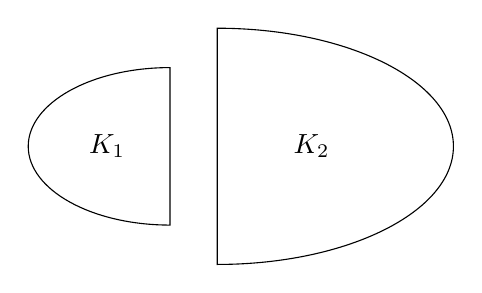
\begin{tikzpicture}[scale=1.0]
		\draw (0,-1.0) arc (-90:-270:1.8cm and 1.0cm) -- (0,1.0) -- cycle;
		\node at (-0.8,0) {$K_1$};
		\draw (0.6,-1.5) -- (0.6,1.5) arc (90:-90:3.0cm and 1.5cm) -- cycle;
		\node at (1.8,0) {$K_2$};
	\end{tikzpicture}
	\caption{}
	\label{fig:9}
\end{figure}

1--4. 在乘积空间中应用 Opial 引理证明弱收敛.

\problemsolutionhead{28}

\runin{-- A --}

1. 正交投影的等价刻画: 自伴性, 范数不超过 1, 核与像正交.

2. 对合算子与正交投影的对应关系.

\runin{-- B --}

1--3. 两个正交投影的可易性与子空间交, 和的正交投影.

\problemsolutionhead{29}

\runin{-- A --}

1--3. 遍历均值序列 $(\sigma_n)$ 弱收敛于不动点.

4--6. 算术平均迭代 $(\mu_n)$ 弱收敛于不动点.

\runin{-- B --}

1--8. 奇算子情形下的 Baillon 强收敛遍历定理.

\problemsolutionhead{30}

\runin{-- A --}

1--3. 摄动双线性形式取极限证明变分不等式解的存在性.

\runin{-- B --}

对上图应用变分不等式得出下半连续凸泛函上的 Stampacchia 定理.

\runin{-- C --}

双线性鞍点问题的 von Neumann 极小化极大定理.

\runin{-- D --}

凸-凹鞍点问题的一般极小化极大定理.
\problemsolutionhead{31}

\runin{-- A --}

3. 注意 $\sum_{i,j}\lambda_i\lambda_j\dual{Av_j}{v_i-v_j}=\frac12\sum_{i,j}\lambda_i\lambda_j\dual{Av_j-Av_i}{v_i-v_j}\le0$.

\runin{-- B --}

2. 对每个 $R>0$, 存在某个 $u_R\in K_R$ 使得对一切 $v\in K_R$, $\dual{Au_R}{v-u_R}\ge0$.
选取 $v=0$, 可见存在与 $R$ 无关的常数 $M$ 使得对一切 $R$, $\norm{u_R}\le M$.固定任何
$R>M$.给定 $w\in K$, 对充分小的 $t>0$ 取 $v=(1-t)u_R+tw$.

3. 取 $K=E$.先证明存在某个 $u\in E$ 使得 $Au=0$.然后用映射 $v\mapsto Av-f$ ($f\in E^\star$ 固定)
代替 $A$.

\problemsolutionhead{32}

2. 对充分小的 $\varepsilon>0$,
\begin{align*}
\phi(u_0)&\le\phi(u_0+\varepsilon v)=\max_{i\in I}\{\abs{u_0-y_i}^2-c_i+2\varepsilon(v,u_0-y_i)\}+O(\varepsilon^2)\\
&=\max_{i\in J(u_0)}\{\abs{u_0-y_i}^2-c_i+2\varepsilon(v,u_0-y_i)\}+O(\varepsilon^2)\\
&\le\phi(u_0)+2\varepsilon\max_{i\in J(u_0)}\{(v,u_0-y_i)\}+O(\varepsilon^2).
\end{align*}

3. 用反证法并应用 Hahn--Banach 定理.

4. 注意对一切 $u,v\in H$,
$\phi(v)-\phi(u)\ge\max_{i\in J(u)}\{\abs{v-y_i}^2-\abs{u-y_i}^2\}\ge2\max_{i\in J(u)}\{(u-y_i,v-u)\}$.

5. 条件 (1) 替换为 $0\in\operatorname{conv}\left(\bigcup_{i\in J(u_0)}\{f'_i(u_0)\}\right)$.

\runin{-- B --}

1. 令 $\sigma_x=\sum_{i\in I}\lambda_ix_i$ 与 $\sigma_y=\sum_{i\in I}\lambda_iy_i$, 我们得到
\begin{align*}
\sum_{j\in I}\lambda_j\abs{\sigma_y-y_j}^2&=-\abs{\sigma_y}^2+\sum_{j\in I}\lambda_j\abs{y_j}^2
=\frac12\sum_{i,j\in I}\lambda_i\lambda_j\abs{y_i-y_j}^2\\
&\le\frac12\sum_{i,j\in I}\lambda_i\lambda_j\abs{x_i-x_j}^2=-\abs{\sigma_x}^2+\sum_{j\in I}\lambda_j\abs{x_j}^2\\
&=-\abs{\sigma_x-p}^2+\sum_{j\in I}\lambda_j\abs{x_j-p}^2.
\end{align*}

2. 把 $u_0$ 写成 $u_0=\sum_{i\in J(u_0)}\lambda_jy_j$.由 B1 的结果,
$\sum_{j\in J(u_0)}\lambda_j\abs{u_0-y_j}^2\le\sum_{j\in J(u_0)}\lambda_j\abs{p-x_j}^2$.由此推出
$\sum_{j\in J(u_0)}\lambda_j\phi(u_0)\le0$, 从而 $\phi(u_0)\le0$.

\runin{注记.} 也可以通过对函数
\begin{equation*}
K(\lambda,\mu)=\sum_{j\in I}\mu_j\abs{\sum_{i\in I}\lambda_iy_i-y_j}^2-\sum_{j\in I}\mu_j\abs{p-x_j}^2
\end{equation*}
应用 von Neumann 极小化极大定理 (见问题 30 第 D 部分) 来建立 $q$ 的存在性.

\runin{-- C --}

1. 令 $K_i=\{z\in H;\ \abs{z-y_i}\le\abs{p-x_i}\}$ 与 $K=\overline{\operatorname{conv}\left(\bigcup_{i\in I}\{y_i\}\right)}$.
须证明 $\left(\bigcap_{i\in I}K_i\right)\cap K\ne\emptyset$.用反证法并归结为有限集 $I$.

2. 考虑由延拓 $S$ 且满足 $T(D(T))\subset\overline{\operatorname{conv}S(D)}$ 的所有压缩映射
$T:D(T)\subset H\to H$ 组成的偏序集.由 Zorn 引理它有极大元 $T_0$, 且 $D(T_0)=H$.

\problemsolutionhead{33}

1. 注意 $\abs{au_n}\le n\abs{u}$, 从而 $u_n\in D(A)$.此外 $\abs{u_n}\le\abs{u}$ 且 $u_n\to u$ 几乎处处.

2. 设在 $L^p$ 中 $u_n\to u$ 且 $au_n\to f$.抽取子序列可以假设 $u_n\to u$ 几乎处处且 $au_n\to f$ 几乎处处.从而 $au=f$.

3. 若 $D(A)=E$, 闭图像定理 (定理  \ref{thm:2.9}) 蕴含存在常数 $C$ 使得对一切 $u\in L^p$,
$\int_\Omega\abs{au}^p\le C\int_\Omega\abs{u}^p$.因此映射 $v\mapsto\int_\Omega\abs{a}^pv$ 是 $L^1$ 上的
连续线性泛函.由定理  \ref{thm:4.14} 存在 $f\in L^\infty$ 使得对一切 $v\in L^1$,
$\int_\Omega\abs{a}^pv=\int_\Omega fv$.因此 $a\in L^\infty$.

4. $N(A)=\{u\in L^p;\ u=0\ \text{几乎处处在}\ [a\ne0]\ \text{上}\}$ 以及
$N(A)^\perp=\{f\in L^{p'};\ f=0\ \text{几乎处处在}\ [a=0]\ \text{上}\}$.

5. $D(A^\star)=\{v\in L^{p'};\ av\in L^{p'}\}$ 且 $A^\star v=av$.

6. 结合闭图像定理与 $a$ 在几乎处处的下界控制.

7. $\sigma(A)$ 落在实质值域闭包中, 两个端点必定属于谱.

8. 若 $a$ 连续, 实质值域与通常值域闭包一致.

9--10. 谱为单点 $\{0\}$ 或算子紧均强迫 $a=0$ 几乎处处.

\problemsolutionhead{34}

\runin{-- A --}

1. 显然 $0\notin\operatorname{EV}(T)$.设 $\lambda\in\operatorname{EV}(T)$ 且 $\lambda\ne0$.
设 $u$ 为相应的特征函数, 从而 $\frac1x\int_0^xu(t)dt=\lambda u(x)$.由此推出 $u\in C^1((0,1])$
且满足 $u=\lambda u+\lambda xu'$.积分这个常微分方程, 可见存在常数 $C$ 使得 $u(x)=Cx^{-1+1/\lambda}$.
由于 $u\in C([0,1])$, 必有 $0<\lambda\le1$.反之任何 $\lambda\in(0,1]$ 是特征值, 相应的特征子空间为
$\CC x^{-1+1/\lambda}$.

3. 我们已知 $[0,1]\subset\sigma(T)\subset[-1,+1]$.对任何满足 $\lambda\notin\{0,1\}$ 的
$\lambda\in\R$, 方程 $Tu-\lambda u=f$ 的显式解由积分给出.

4. 直接计算给出当 $q>1$ 时 $\norm{T_\varepsilon u-Tu}_{L^q(0,1)}\le\dfrac{\varepsilon^{1/q}}{(q-1)^{1/q}}\norm{u}_{L^\infty(0,1)}$,
当 $q=1$ 时 $\norm{T_\varepsilon u-Tu}_{L^1(0,1)}\le\varepsilon\log(1+1/\varepsilon)\norm{u}_{L^\infty(0,1)}$.
从而 $\norm{T_\varepsilon-T}\to0$.显然 $T_\varepsilon\in\KK(E,F)$, 从而 $T\in\KK(E,F)$.

\runin{-- B --}

1. 把 $Tu(x)$ 写成 $Tu(x)=\int_0^1u(xs)ds$, 从而 $(Tu)'(x)=\int_0^1u'(xs)sds$.

2. $\operatorname{EV}(T)=(0,1/2]\cup\{1\}$.

3. $\sigma(T)=[0,1/2]\cup\{1\}$.

\runin{-- C --}

1. 分部积分并应用 Hölder 不等式建立 Hardy 不等式.

2. 由稠密性推广到一般的 $u\in E$.

3. $\operatorname{EV}(T)=(0,p/(p-1))$.

4. $\norm{T}_{\LL(E)}=\dfrac{p}{p-1}$.$T$ 不是紧算子.

5. $\sigma(T)=[0,p/(p-1)]$.

6. $(T^\star v)(x)=\int_x^1\dfrac{v(t)}{t}dt$.

7. 由 Ascoli 定理与范数逼近证明 $T\in\KK(E,F)$.

\problemsolutionhead{35}

\runin{-- A --}

1. 显然 $\norm{T^\star T}\le\norm{T}^2$.另一方面, $\abs{Tx}^2=(Tx,Tx)=(T^\star Tx,x)\le\norm{T^\star T}\abs{x}^2$.
故 $\norm{T}^2\le\norm{T^\star T}$.

2. 由归纳法 $\norm{T^{2^k}}=\norm{T}^{2^k}$.对任何整数 $N$, 选取满足 $N\le2^k$ 的 $k$,
写出 $\norm{T}^{2^k}=\norm{T^{2^k}}\le\norm{T^N}\norm{T}^{2^k-N}$, 从而 $\norm{T}^N\le\norm{T^N}$.

\runin{-- B --}

1. 利用假设 (1) 与 (2) 交替控制相邻算子对的范数.

2--3. 求和并取 $2N$ 次方根, 令 $N\to\infty$ 建立 Cotlar 引理的不等式.

\problemsolutionhead{36}

1. $R_k$ 闭是因为 $(I-T)^k=I-S$, 其中 $S\in\KK(E)$, 应用定理  \ref{thm:6.6}.

2. 降链平稳性.

4. 对偶关系的维数等式 $\operatorname{codim}R_k=\dim N_k$.

5. $R_p\cap N_p=\{0\}$ 且 $R_p+N_p=E$.

6. $(I-T)$ 限制在 $R_p$ 上是满同构.

7. 自伴算子下平方等于零蕴含本身为零, 故 $p=1$.

\problemsolutionhead{37}

10. 由第 9 问, $\nu_k^{(n)}$ 关于 $n$ 单调不减且 $\nu_k^{(n)}\le\mu_k$.利用投影算子强收敛到恒等
算子的性质, 逼近特征向量张成的有限维子空间, 建立 $\liminf\nu_k^{(n)}\ge\mu_k$.

\problemsolutionhead{38}

\runin{-- A --}

2. 对算子 $(I_F+K)$ 应用第 1 问.

3. 由有限余维子空间性质与对偶闭域定理证明.

\runin{-- B --}

对合伴随算子对偶转化.

\runin{-- C --}

1--13. Fredholm 算子的指标性质: 伴随算子的反号指标, 有限秩与紧摄动不变性, 乘积指标可加性
$\operatorname{ind}(T_2\circ T_1)=\operatorname{ind}T_1+\operatorname{ind}T_2$.

\runin{-- D --}

1. 有限维情形 $\operatorname{ind}T=\dim E-\dim F$.

2. 移位算子的 Fredholm 性与指标计算.
\problemsolutionhead{41}

\runin{-- A --}

1. 反设 $a\in(\operatorname{Int}P)\cap(-P)$.由习题 1.7, $0=\frac12a+\frac12(-a)\in\operatorname{Int}P$,
这蕴含 $P=E$, 与假设 (2) 矛盾.

2. 反设存在 $P$ 中的序列 $(x_n)$ 使得 $x_n+u\to0$.由于 $(x_n+u)-u=x_n\in P$, 取极限得到
$-u\in P$, 矛盾于第 1 问.

3. 显然 $u\ne0$ (因为由 (2), $0\notin\operatorname{Int}P$).由 (3) 有 $Tu\in\operatorname{Int}P$,
从而对某个 $\rho>0$ 有 $B(Tu,\rho)\subset P$.选取 $0<r<\rho/\norm{u}$.

4. 由于 $\lambda x=T(x+u)\ge Tu\ge ru$, 有 $\frac\lambda r x\ge u$.若归纳假设
$(\lambda/r)^nx\ge u$, 则有 $(\lambda/r)^nTx\ge Tu$, 从而 $(\lambda/r)^n(\lambda x-Tu)\ge Tu\ge ru$.
因此 $(\lambda/r)^n\lambda x\ge ru$, 即 $(\lambda/r)^{n+1}x\ge u$.另一方面,
$\lambda x=T(x+u)\in\operatorname{Int}P$, 这蕴含 $\lambda>0$ (由第 1 问).若 $0<\lambda<r$,
令 $n\to\infty$ 取极限将得到 $-u\in P$, 这不可能.

5. 映射 $x\mapsto(x+u)/\norm{x+u}$ 在 $P$ 上显然连续 (由第 2 问).由于 $T\in\KK(E)$,
$F(P)\subset T(B_E)\subset K$.应用 Schauder 不动点定理 (见习题 6.26).

6. 把 $u$ 换成 $\varepsilon u$ 时, 第 2 问中的常数 $\alpha$ 可能改变, 但第 3 问中的常数 $r$ 保持不变.

7. 有 $\lambda_\varepsilon\norm{x_\varepsilon}=\norm{T(x_\varepsilon+\varepsilon u)}\le\norm{T}\norm{x_\varepsilon+\varepsilon u}$,
因此 $\norm{x_\varepsilon}\le\norm{T}$.抽取子序列 $\varepsilon_n\to0$, 设 $\lambda_{\varepsilon_n}\to\mu_0$,
$Tx_{\varepsilon_n}\to\ell$, 得出 $x_{\varepsilon_n}\to x_0$, 其中 $x_0\in P$,
$\mu_0=\norm{x_0}\ge r$ 且 $Tx_0=\mu_0x_0$, 由 (3) 知 $x_0\in\operatorname{Int}P$.

\runin{-- B --}

1. 集合 $\Sigma=\{s\in[0,1];\ (1-s)a+sb\in P\}$ 是闭区间.由习题 1.7, $\sigma=\max\{s;\ s\in\Sigma\}$
具有所要求的性质.

2. 不能有 $\mu=0$ (否则 $0\in\operatorname{Int}P$), 也不能有 $\mu<0$ (否则 $-x\in(\operatorname{Int}P)\cap(-P)$).
故 $\mu>0$, 从而 $x\in\operatorname{Int}P$ 且 $-x\notin P$.注意 $x_0$ 与 $x$ 扮演对称角色.
令 $y=x_0-\tau_0x$, 其中 $\tau_0=\tau(x_0,-x)$.则 $y\in P$ 且 $y\ne0$.因此 $Ty\in\operatorname{Int}P$.
但 $Ty=\mu_0x_0-\tau_0\mu x$, 从而 $x_0+\dfrac{\tau_0\mu}{\mu_0}(-x)\in\operatorname{Int}P$.由 $\tau_0$
的定义得出 $\dfrac{\tau_0\mu}{\mu_0}<\tau_0$, 从而 $\mu<\mu_0$.互换 $x_0$ 与 $x$ 的角色导出 $\mu_0<\mu$.
矛盾.因此存在 $m>0$ 使得 $x=mx_0$, 进而 $\mu=\mu_0$.

3. 若 $x\in P$ 或 $-x\in P$, 由第 2 问可得结论的第一种情形.故可设 $x\notin P$ 且 $-x\notin P$.
通过分别对 $\mu>0$ 与 $\mu<0$ 考虑 $\tau_0$ 与 $\tilde\tau_0$, 证明 $\abs{\mu}<\mu_0$.

4. 几何重数为 1.

5. 鉴于问题 36, 只须证明 $N((T-\mu_0I)^2)=N(T-\mu_0I)$.反设存在满足 $Tx-\mu_0x=\alpha x_0$
($\alpha\ne0$) 的 $x$, 迭代计算得出当 $n\to\infty$ 时产生矛盾.

\problemsolutionhead{42}

\runin{-- A --}

1. 验证 $0\notin C$, 且对一切 $x\in C$, $\norm{Tx-Tx_0}\le\frac12\norm{Tx_0}$, 从而
$\norm{Tx}\ge\frac12\norm{Tx_0}$.由此推出 $0\notin\overline{T(C)}$.

2--3. 利用假设 \eqref{eq:prob42.1} 在每个非零点附近找到满意的算子 $S_y$ 并由连续性拓展到邻域.

4--6. 提取有限覆盖, 构造连续非线性映射 $F$, 并由 Schauder 不动点定理得出不动点 $\xi$.

7--8. 由不动点算子构造紧算子 $U$, 证明其核有限维且非平凡, 并在 $T$ 下不变.

9. 在 $\R^2$ 中考虑旋转算子.

\runin{-- B --}

把单算子代数 $\mathcal{A}$ 换成与 $T$ 对易的算子 $R$ 生成的代数 $\mathcal{B}$, 所有论证平行成立.

\problemsolutionhead{43}

1. 计算 $\abs{T(u+v)}^2$ 展开并作内积实部消去.

2. 利用正规性得出 $N(T^\star-\mu I)=N(T-\mu I)$, 进而正交.

3. 闭域定理与正规性给出正交补恒等式.

4--6. 证明 $R(T)=R(T^\star)$.

7--8. 归纳证明高阶幂范数等式 $\norm{T^p}=\norm{T}^p$.

9. 核的降链在一步即平稳: $N(T^2)=N(T)$.

\problemsolutionhead{44}

\runin{-- A --}

2. 由等距定义展开 $\abs{T(u+v)}^2$ 证明 $T^\star\circ T=I$.

3. 酉算子, 伴随算子等距性与可逆性之间的五重等价.

4. 经典反例: $\ell^2$ 上的右移位算子.

5. $T\circ T^\star=P_{R(T)}$.

6. 酉算子谱落在 $\{-1,+1\}$ 中, 非酉等距谱填满整个闭区间 $[-1,+1]$.

7. 紧等距强迫空间有限维.

8--11. 斜自伴算子性质与其 Cayley 变换的酉性.

\runin{-- B --}

1--12. 极分解定理 $T=U\circ P$ 的存在性, 唯一性与紧算子的谱分解展开.

\problemsolutionhead{45}

12. 对常系数热方程显式求解 Green 函数, 利用初等函数估计下界, 再通过变量代换推广到一般 Sturm--Liouville 算子.

\problemsolutionhead{46}

12. 极小化序列在 $H_0^1(I)$ 中有界, 弱极限与紧嵌入结合证明下确界可达.

\problemsolutionhead{47}

\runin{-- A --}

2--3. 平移尖峰逼近列给出上确界为 1, 但无法由 $W^{1,1}$ 函数达到.

4--5. 两端积分控制给出 $W_0^{1,1}$ 的最佳常数 $1/2$.

6. $p>1$ 时通过弱紧性证明最佳常数可达.

\runin{-- B --}

1--5. 通过正交特征函数展开与 Sturm--Liouville 特征值求解出最佳常数为 $1/\pi$.

\runin{-- C --}

1--4. Fubini 定理给出加权导数积分控制, 证明常数 $1/2$ 是最优的但不可达.

\problemsolutionhead{49}

7--11. 极小化比值确定第一特征函数 $w_0$, 取绝对值后由强极大值原理证明严格正性, 并由检验函数法证明特征子空间的一维性.

\problemsolutionhead{50}

2--6. 变分极小化构造非平凡非负解, 强极大值原理给出正性.

8--10. 严格凸泛函变换证明正解唯一性, 从而原问题恰有两个对称极小元.

\problemsolutionhead{51}

1--3. 调和振子二次增长势能 $p(x)=x^2$ 的完备化空间 $V$, 证明形式强制.

4--6. 证明 Green 算子自伴紧, 从而存在离散谱.

7--8. Hermite 多项式基与其特征值 $\lambda_n=2n+1$.
